\documentclass[../bericht.tex]{subfiles}

\begin{document}

  \chapter{Einleitung}

    Die Sekunde ist das $9.192.631.770$-fache der Periodendauer der dem Übergang zwischen den beiden Hyperfeinstrukturniveaus des Grundzustandes von Atomen des Nuklids $\mathrm{^{133}Cs}$ entsprechenden Strahlung - so die Definition nach dem SI-Einheitensystem. Genau diese Periodendauer soll im folgenden Versuch gemessen werden. Hierzu werden sowohl die Feinstruktur als auch die Hyperfeinstruktur erklärt und mittels der dopplerfreien Spektroskopie der Übergang aufgelöst.


  \chapter{Versuch}

    \section{Feinstruktur}
    \label{sec:feinstruktur}

      Nach dem semiklassischen Atommodell kreisen die negativ geladenen Elektronen auf einer Kreisbahn um den positiv geladenen Atomkern. Die Rotation stellt einen Kreisstrom dar. Dieser erzeugt ein magnetisches Dipolmoment, welches über den Bahndrehimpuls $\vec{l}$ ausgedrückt werden kann. Gemä\ss dem \textsc{Stern-Gerlach}-Experiment (und anderen Experimenten) haben Elektronen ein weiteres magnetisches Dipolmoment inne, welchem der Spin $\vec{s}$ zugrunde liegt. Die beiden magnetischen Momente wechselwirken in der sogenannten \textit{Spin-Bahn-Kopplung}. Je nach Einstellung des Elektronenspins (\textit{Spin-up}/ \textit{Spin-down}, d.h. für die $z$-Komponente des Spins $s_z=\pm \frac{\hslash}{2}$) ergibt sich eine positive, bzw. negative Energiekorrektur $\Delta E_{l,s}$, die sogenannte \textit{Spin-Bahn-Kopplungsenergie}.

      Bei der mathematischen Betrachtung sind für die \textit{Feinstrukturaufspaltung} außerdem relativistische Effekte zu beachten. Auf der Umlaufbahn um den ruhenden Kern dreht sich das Elektron einmal um die zum Drehimpuls parallele Achse. Dies führt zu einer Korrektur der kinetischen Energie $\Delta E_\mathrm{rel}$.

      Zuletzt muss der \textit{\textsc{Darwin}-Term} $\Delta E_\mathrm{Darwin}$ berücksichtigt werden. Als Folge der relativistischen Zitterbewegung des Elektrons auf seiner Kreisbahn verkompliziert sich die elektrostatische Wechselwirkung zwischen Elektron und Atomkern.
      \medskip

      Die gesamte Energiekorrektur
      \begin{equation*}
        \Delta E = \Delta E_{l,s} + \Delta E_\mathrm{rel} + \Delta E_\mathrm{Darwin}
      \end{equation*}
      führt zur sogenannten \textit{Feinstrukturaufspaltung}.
      \medskip

      Zur Beschreibung dieser Zustände wird der Gesamtdrehimpuls $\vec{j}=\vec{l}+\vec{s}$ mit der zugehörigen gutartigen Gesamtdrehimpulsquantenzahl $j$ eingeführt. Letzte kann die Werte
      \begin{equation*}
        j=+\frac{1}{2} \quad\text{für}\quad l=0
      \end{equation*}
      und
      \begin{equation*}
        j=l\pm \frac{1}{2}\quad\text{für}\quad l>0
      \end{equation*}
      annehmen. Somit spalten alle Zustände mit $l>0$ in zwei \textit{Feinstrukturniveaus} auf.


    \section{Hyperfeinstruktur}
    \label{sec:hyperfeinstruktur}

      Analog zum Spin des Elektrons wird auch dem räumlich ausgedehnten Atomkern ein Spin zugeordnet, der sogenannte \textit{Kernspin} $\vec{I}$. Das dem Spin zugeordnete magnetische Moment des Kerns wechselwirkt mit dem Gesamtspin des Elektrons $\vec{j}$. Wiederum kommt es je nach Ausrichtung des Kernspins zu einer Energiekorrektur welche positiv und negativ ausfallen kann. Die Projektion auf die $z$-Richtung von $\vec{I}$ kann die $(2I + 1)$ Werte
      \begin{equation*}
        I_z=m_I \cdot \hslah\quad\text{mit}\quad -I\le m_I \le +I
      \end{equation*}
      annehmen. Zur Zustandsbeschreibung wird nun der Gesamtdrehimpuls des Atoms $\vec{F}=\vec{j}+\vec{I}$ mit der zugehörigen gutartigen Quantenzahl $F$,
      \begin{equation*}
        |j-I| \le F\le |j + I|
      \end{equation*}
      eingeführt. Die \textit{Feinstrukturniveaus} spalten also in
      \begin{equation*}
        \begin{cases}
            (2I+1), & I<j\\
            (2j+1), & j<I
        \end{cases}
      \end{equation*}
      \textit{Hyperfeinstrukturniveaus} auf. Aufgrund der im Vergleich zum Elektron extrem großen Masse des Kerns
      \begin{equation*}
        m_\mathrm{Kern}\approx Z\cdot 1836 \cdot m_\mathrm{e},
      \end{equation*}
      mit der Kernladungszahl $Z$, ist die Energieaufspaltung in Folge der \textit{Hyperfeinstruktur} sehr klein. Um diese zu messen ist also extrem schmalbandiges Licht notwendig, welches gleichzeitig so intensiv sein muss, dass ein messbares Signal entsteht. Weil Monochromatoren zu breitbandig sind, erfordert das Experiment also einen Laser.


    \section{Termschema von Cäsium}
    \label{sec:termschema-caesium}

      Im Versuch wird das Nuklid $\mathrm{^{133}Cs}$ verwendet. Dessen relevantes Termschema mit Feinstrukturaufspaltung und Hyperfeinstrukturaufspaltung ist in \cref{fig:feinstruktur-hyperfeinstruktur} abgebildet. Die Kernspinquantenzahl ist $I=\frac{7}{2}$. Weiter sind die erlaubten Übergänge als direkte Folge von anregender Strahlung eingezeichnet (keine Relaxationen!). Für diese ist zu beachten, dass anregende Photonen einen Spin von $1$ tragen. Es gelten die Übergangsregeln
      \begin{equation*}
        \Delta l = 1\quad \text{und}\quad \Delta F = -1,0,+1.
      \end{equation*}

      \begin{figure}[tb]
        \centering
        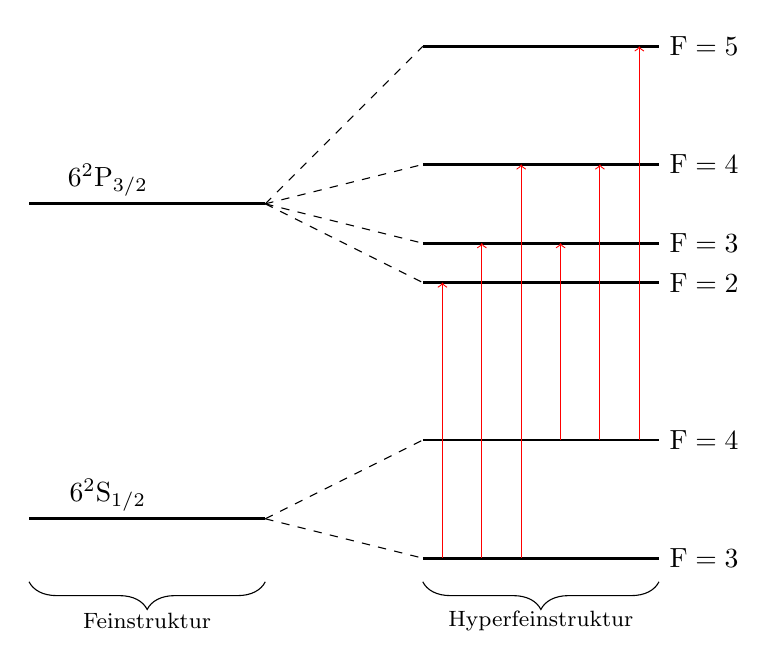
\begin{tikzpicture}
          % angeregte Niveaus
          \node at (1,4.3) {$\mathrm{6^2P_{3/2}}$};
          \draw[line width=1pt] (0,4)--(3,4);
          \draw[line width=1pt] (5,6)--(8,6) node[anchor=west] {$\mathrm{F=5}$};
          \draw[line width=1pt] (5,4.5)--(8,4.5) node[anchor=west] {$\mathrm{F=4}$};
          \draw[line width=1pt] (5,3.5)--(8,3.5) node[anchor=west] {$\mathrm{F=3}$};
          \draw[line width=1pt] (5,3)--(8,3) node[anchor=west] {$\mathrm{F=2}$};
          \draw[dashed] (3,4)--(5,6);
          \draw[dashed] (3,4)--(5,4.5);
          \draw[dashed] (3,4)--(5,3.5);
          \draw[dashed] (3,4)--(5,3);
          % Grundzustand Niveaus
          \node at (1,0.3) {$\mathrm{6^2S_{1/2}}$};
          \draw[line width=1pt](0,0)--(3,0);
          \draw[line width=1pt] (5,1)--(8,1) node[anchor=west] {$\mathrm{F=4}$};
          \draw[line width=1pt] (5,-0.5)--(8,-0.5) node[anchor=west] {$\mathrm{F=3}$};
          \draw[dashed] (3,0)--(5,1);
          \draw[dashed] (3,0)--(5,-0.5);
          % Übergänge
          % Unterer Grundzustand
          \draw[color=red, ->] (5.25,-0.5)--(5.25,3);
          \draw[color=red, ->] (5.75,-0.5)--(5.75,3.5);
          \draw[color=red, ->] (6.25,-0.5)--(6.25,4.5);
          % Oberer Grundzustand
          \draw[color=red, ->] (6.75,1)--(6.75,3.5);
          \draw[color=red, ->] (7.25,1)--(7.25,4.5);
          \draw[color=red, ->] (7.75,1)--(7.75,6);
          % Fein- und Hyperfeinstruktur
          \draw [decorate,decoration={brace,mirror,amplitude=10pt}] (0,-0.8) -- (3,-0.8) node [black,midway,yshift=-14pt] {\footnotesize Feinstruktur};
          \draw [decorate,decoration={brace,mirror,amplitude=10pt}] (5,-0.8) -- (8,-0.8) node [black,midway,yshift=-14pt] {\footnotesize Hyperfeinstruktur};
        \end{tikzpicture}
        \caption{Termschema von $\mathrm{^{133}Cs}$ ($I=\frac{7}{2}$) mit Feinstruktur und Hyperfeinstruktur. Die erlaubten Anregungsübergänge sind rot markiert. }
        \label{fig:feinstruktur-hyperfeinstruktur}
      \end{figure}


    \section{Diodenlaser}
    \label{sec:diodenlaser}


      \subsection{Linienbreite}
      \label{subsec:linienbreite}


    \section{Transmissionsspektroskopie}
    \label{sec:transmissionsspektroskopie}


    \section{Dopplerfreie Spektroskopie}
    \label{sec:dopplerfreie-spektroskopie}


      6 statt 3 erwartete Peaks


      \subsection{Cross-over Resonanzen}
      \label{subsec:cross-over-resonanzen}

        genau in der mittels


    \section{Zeeman-Effekt}
    \label{sec:zeeman-effekt}

      nicht observierbar!










\end{document}
